
\documentclass{../oxmathproblems}
\usepackage{blindtext}
\usepackage{hyperref}
\usepackage{geometry}

\course{ITAM - Estadística 1}
\oxfordterm{Assignment 04}
\sheetnumber{1}
\sheettitle{}
\extrawidth{2cm}
\begin{document}

\begin{questions}

\question\textbf {Variable aleatorias discretas.}

\begin{itemize}
\item  a) Continua 
\item  b) Discreto 
\item  c) Continua 
\item  d) Discreta 
\item  e) Continua 
\end{itemize}

\question\textbf {Variable aleatorias discretas.}

\begin{itemize}
\item  a) 

\text{Para determinar} P(x=4) 
\text{sabemos que} 
        $$ \sum_x p(x)= 1 $$ 
\text{entonces}
$$ P(x=4) = .10$$

\item  b) 
\text{Para determinar el valor esperado de x, sabemos que} 
$$ \mu = E(x)= \sum_x xp(x)$$

\text{entonces} 

$$ \mu = E(x)= (0)(0.10)+ (1)(0.40)+ ... +(5)(0.05) = 1.90 $$

\text{Ahora, para determinar la varianza }  ( $\sigma^2_x$) 
\text{sabemos que} 
  $$ \sigma^2_x = E[x^2]-E[x]^2 $$
  
\text{Entonces: } 
$$ E[x^2] = (0)^2(0.10)+ (1)^2(0.40)+ ... +(5)^2(0.05)= 5.4 $$ 

$$ E[x]^2 = (1.9)^2 = 3.61  $$

 $$ \sigma^2_x = E[x^2]-E[x]^2 = 5.4 - 3.61 = 1.79 $$

\text{Para la desviación estándar ($\sigma_x$), tenemos que  $\sigma_x$ = $\sqrt\sigma^2_x$ }

$$ \sigma_x = \sqrt{1.79} = 1.34 $$ 
\end{itemize}

\question 
\text{Su ganancia x puede tomar uno de dos valores.} \text {O bien} \text {perderá 20 ( es decir, su " ganancia" será de -20)}
\text {o ganará 23 980, con probabilidad de 7998/8000 y  2/8000, respectivamente.}

 \text {Entonces, tenemos que:}

 \begin{center}
\begin{tabular}{ |c|c| } 
 \hline
 \textbf{x} & \textbf{p(x)} \\ 
 \hline
 -20 & 7998/8000 \\
 23980  & 2/8000 \\
 \hline
\end{tabular}
\end{center} 

\text {La ganancia esperada será }

$$ \mu = E(x)= \sum_x xp(x)$$
 
   $$  = (-20)(\frac{7998}{8000}) + (23 980)(\frac{2}{8000}) = -14 $$ 

\question  
\text {El diagrama de árbol muestra los eventos siguientes:}
$$ \text { R:se escoge un juguete rojo} $$ 
$$ \text { G:se escoge un juguete verde} $$ 

$$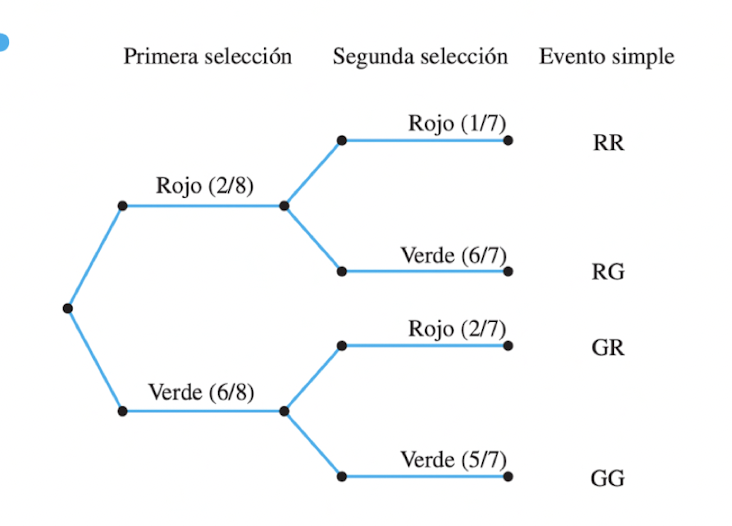
\includegraphics[width=0.6\textwidth]{A04-arbol}$$

\question  

\begin{itemize}
\item  a) El salario medio por hora 
$$ \mu = E(x)= \sum_x x *(1/n)$$

\text{Entonces} 
$$ \mu_x = E(x)= 10.33$$

\item  b) El número promedio de años de experiencia 
$$ \mu_y = E(y)= 4.5$$

\item  c) Varianza de "x" y de "y": 
\text{ Ahora, para determinar la varianza para x}  ( $\sigma^2_x$) 
\text{sabemos que} 
  $$ \sigma^2_x = E[x^2]-E[x]^2 = 13.76 $$
  
\text{Ahora, para determinar la varianza  de y}  ( $\sigma^2_y$) 
\text{sabemos que} 
  $$ \sigma^2_y = E[y^2]-E[y]^2 = 2.91 $$

\text{Para la desviación estándar de "x" y de "y". }  
  \text{Para la desviación estándar ($\sigma_x$), tenemos que  $\sigma_x$ = $\sqrt\sigma^2_x$ }

$$ \sigma_x = \sqrt(13.76) = 3.71$$ 

  \text{Ahora, para y}
$$ \sigma_y = \sqrt(1360.46) = 36.88$$   
\end{itemize}



\end{questions} 

\end{document}


